%--Pr�ambel
\documentclass{beamer}
\usepackage{graphicx}

\usepackage[latin1]{inputenc}

% upright differenzial symbol with good spacing included!!!
\makeatletter
\providecommand*{\diff}%
	{\@ifnextchar^{\DIfF}{\DIfF^{}}}
\def\DIfF^#1{%
	\mathop{\mathrm{\mathstrut d}}%
		\nolimits^{#1}\gobblespace
}
\def\gobblespace{%
	\futurelet\diffarg\opspace}
\def\opspace{%
	\let\DiffSpace\!%
	\ifx\diffarg(%
		\let\DiffSpace\relax
	\else
		\ifx\diffarg\{%
			\let\DiffSpace\relax
		\else
			\ifx\diffarg\{%
				\let\DiffSpace\relax
			\fi\fi\fi\DiffSpace}


%Verwendetes Template
\usetheme{Berlin}

%--Daten der Titelseite
\title{Presentation\\ \textbf{GEN-UE6} Group 5 Team F}
\author{Severin Wolf, Maximilian Seidler}
\date{\today}

%--Hauptinhalte
\begin{document}

%%% Titelseite anzeigen
\frame{\titlepage}

\begin{frame}
\frametitle{Table of Contents}
\tableofcontents
\end{frame}

%%% und eine leere folie
\section{Specification} 
\begin{frame}
\frametitle{Specification}
\begin{figure}[!htb]
\begin{minipage}{0.55\textwidth}
  \centering
  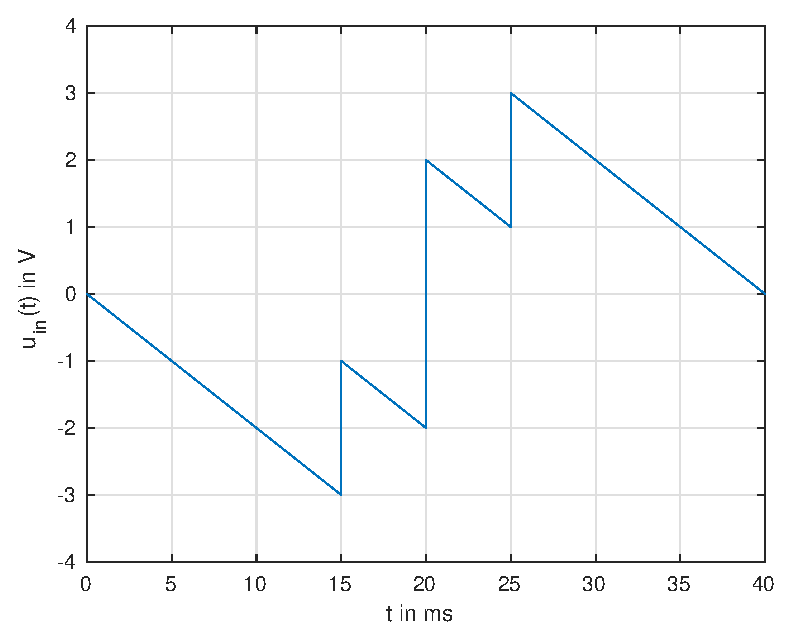
\includegraphics[width=1\textwidth]{../latex/Figures/inputsignal.eps}
  \caption{Input Signal}
  \label{fig:input}
\end{minipage}\hfill
\begin{minipage}{0.39\textwidth}
  \centering
  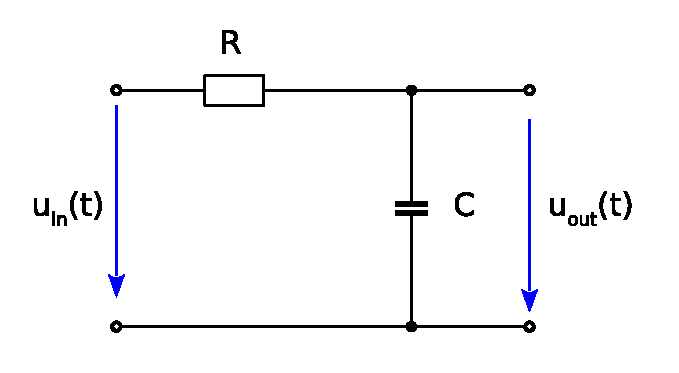
\includegraphics[width=1\textwidth]{../latex/Figures/filter.eps}
  \caption{Filter-Circuit}
  \label{fig:filter}
\end{minipage}
\end{figure}
\end{frame}

\section{Fourier Series}
\begin{frame}
\frametitle{Drichlet conditions}
  \begin{itemize}
    \item $f(t)$ is a function
    \item $f(t)$ has a finite number of discontinuities in a periodic time interval
    \item $f(t)$ has a finite number of maxima and minima in a periodic interval
    \item  $f(t)$ must be absolutely integrable,  $\int_{t_0}^{t_0+T} \left| f(t) \right| \diff t$
  \end{itemize}
\end{frame}


\begin{frame}
\frametitle{General Formular}
  The Fourier Series:
    \[
      f(t)  = a_{0} + \sum_{k=1}^{\infty}(a_{k}\cos k\omega t + b_{k} \sin k\omega t)
    .\] 
\end{frame}

\begin{frame}
\frametitle{Coefficients}
  \begin{itemize}
    \item<1-> DC-term $a_{0} = \frac{1}{T} \int_{0}^{T} f(t) \diff t$. In our
      case, $a_{0} = 0$, since $f$ the area above and below  $x=0$ is equal. 
    \item<2-> The cosine coefficients $a_{k} = \frac{2}{T}\int_{0}^{T} f(t) \cos k \omega t \diff t$ are
      also $0$, because  $f(t) = -f(-t)$.
    \item<3-> The sine coefficients
      \[
	b_{k} = \frac{2}{T} \int_{0}^{T} f(t) \sin k \omega t \diff t
      ,\] 
      need to be calculated.
  \end{itemize}
\end{frame}

\begin{frame}
\frametitle{Trapezoidal rule}
With 
\[
  \int_{a}^{b} f(t) \diff t = \frac{b-a}{n} \left[\frac{f(a)}{2} + \sum_{i=1}^{n-1}
    f \left( a + i \frac{b-a}{n} \right) + \frac{f(b)}{2} \right]
\]
we can approcimate integrals, using $n$ trapezoidal pices, fittet to the function. In Matlab there
is the function trapz(), which uses that formular. 
\end{frame}
\begin{frame}
\frametitle{Input Signal matlab}
  To get enough points for a good approximation:
  \begin{figure}
    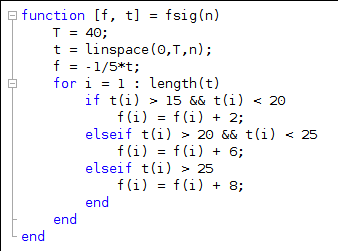
\includegraphics[scale=0.6]{../latex/Figures/funcsig_matlab.png}
\end{figure}
\end{frame}


\begin{frame}
\frametitle{Fourier series, numerically  with matlab}
  \begin{figure}
    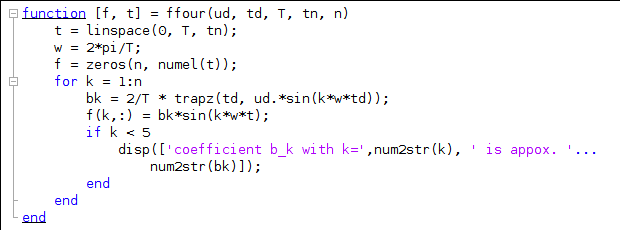
\includegraphics[scale=0.4]{../latex/Figures/funcfour_matlab.png}
  \end{figure}
  Let td and td be the return of our fsig function, to get:
  \begin{figure}
    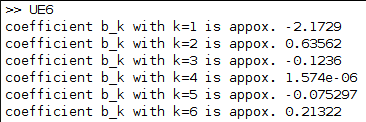
\includegraphics[scale=0.4]{../latex/Figures/matlab_out.png}
  \end{figure}
\end{frame}

\begin{frame}
  The first four \textbf{nonzero} harmonic are where $k$ is  $2, 3, 5$ and  $6$.
  \[
    b_{1} = -2.1729, \, b_{2} = 0.6356, \, b_{3} = -0.1236 
  \]
  \[
    b_{4} = 0, \, b_{5} = -0.0752, \, b_{6} = 0.2132
  .\]   
\end{frame}

\begin{frame}
\frametitle{Frequencies}
  For each $k$ of the fourier series, the frequency of that harmonic can be calculated via $f_{k} =
  k \frac{1}{T}$. For the first five sines, that yields:
  \[
    f_{1} = 25Hz, \quad f_{2} = 50Hz, \quad f_{3} = 75Hz, \quad
  \]
  \[
    f_{5} = 125Hz, \quad f_{6} = 150Hz
  .\] 
\end{frame}

\begin{frame}
\frametitle{Plot, $n=6$}
\begin{figure}
  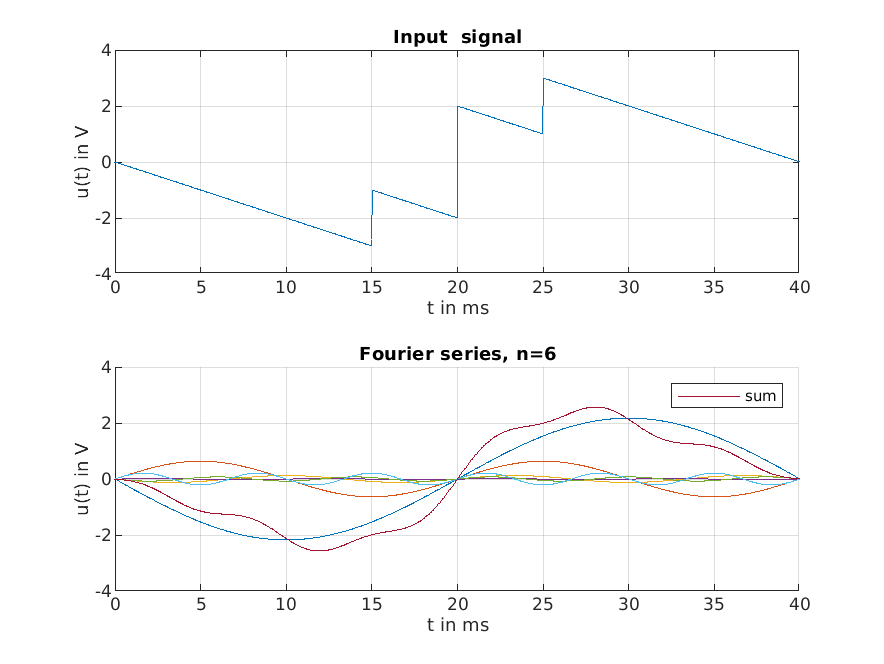
\includegraphics[scale=0.55]{../latex/Figures/fourier_n5.png} 
\end{figure}
\end{frame}

\begin{frame}
\frametitle{Plot, $n=250$}
\begin{figure}
  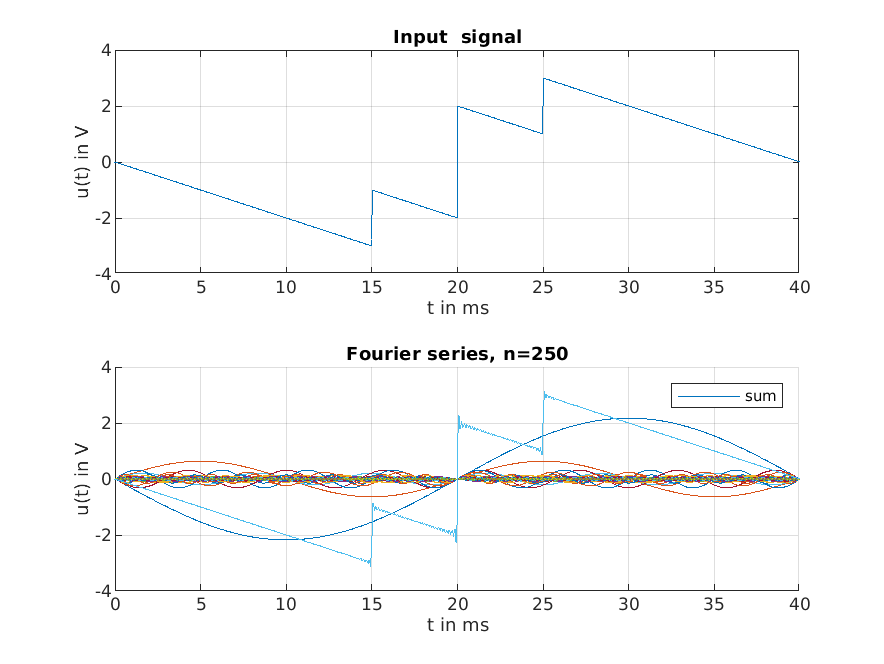
\includegraphics[scale=0.55]{../latex/Figures/fourier_n250.png} 
\end{figure}
\end{frame}

\begin{frame}
\frametitle{Convergence}
\begin{itemize}
  \item converges to $f(t)$, for all points $t$, where $f(t)$ is continous.
  \item $\frac{f(t+) + f(t-)}{2}$ for points $t$, where does a conditional jump.
    
\end{itemize}
\end{frame}

\section{RC Filter}

\begin{frame}
  \frametitle{Lowpass-Filter}
  \begin{figure}
    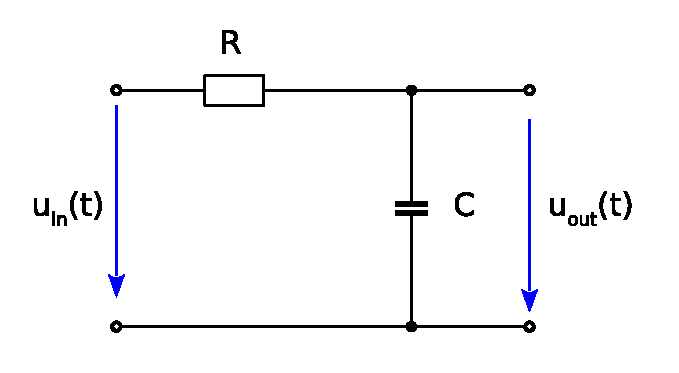
\includegraphics[scale=0.6]{../latex/Figures/filter.eps}
  \end{figure}
  \begin{itemize}
    \item Frequencies higher than fourth nonzereo harmonic should be cut off
    \item determination of the capacity $C$
  \end{itemize}
\end{frame}
\begin{frame}
  \frametitle{Determination of $C$}
  \begin{itemize}
    \item $\Omega$ is the cut off frequency ($|H(j\Omega)|_{dB} = -3dB$)
    \item $\Omega \overset{!}{=} \omega_4$
    \item $C = 0.8\mu F$
  \end{itemize}
\end{frame}
\begin{frame}
  \frametitle{Transfer function $\underline{H}(j\omega)$}
  \begin{itemize}
    \item transformation of filter network into frequency domain
    \item $\underline{H}(j\omega) = \frac{\underline{U}_{out}}{\underline{U}_{in}}.$
    \item $\underline{H}(j\omega) = \frac{1}{1 + j\frac{\omega}{\Omega}}$
    \item add that to the fourier series
    \item $u_{out} = b_k \cdot |H(jk\omega)| \cdot \sin(k\omega t + arg\{H(jk\omega)\})$
  \end{itemize}
\end{frame}
\begin{frame}
  \frametitle{Plot of the output signal}
  \begin{figure}
    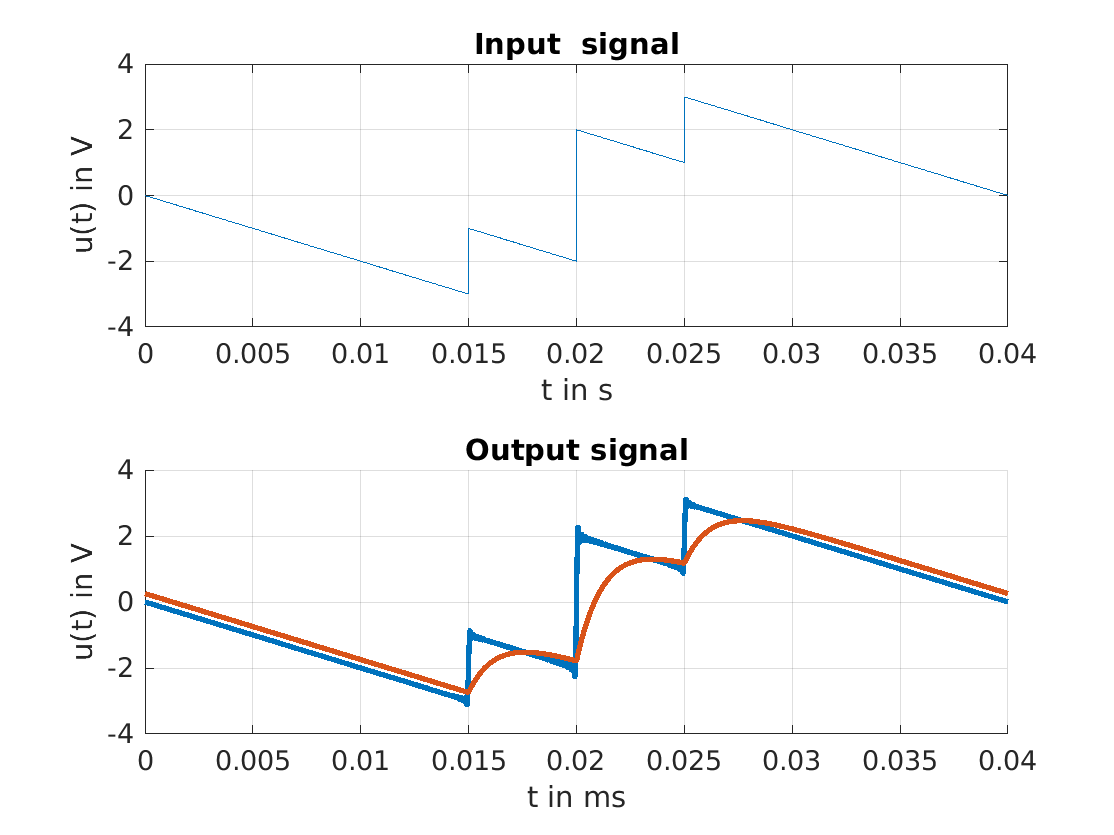
\includegraphics[scale=0.5]{../latex/Figures/output_signal.png}
  \end{figure}
\end{frame}
\end{document}
